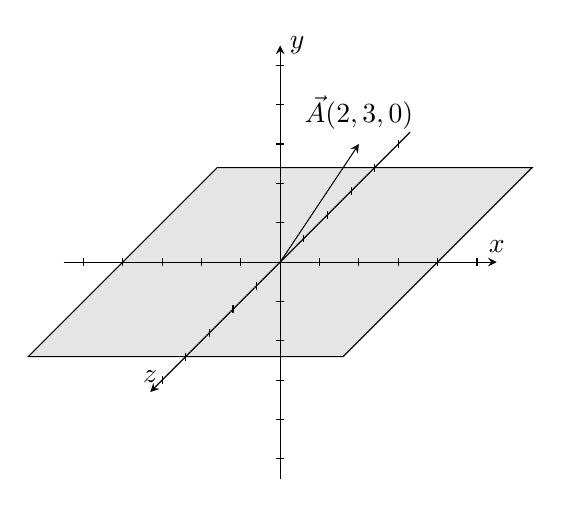
\begin{tikzpicture}[x=0.5cm,y=0.5cm,z=0.3cm,>=stealth]
\coordinate (O) at (0,0,0);
\coordinate (A) at (2,3,0);
\coordinate (P1) at (-5,-5,0);
\coordinate (P2) at (-5, 5,0);
\coordinate (P3) at ( 5, 5,0);
\coordinate (P4) at ( 5,-5,0);
% The axes
\draw[->] (xyz cs:x=-5.5) -- (xyz cs:x= 5.5) node[above] {$x$};
\draw[->] (xyz cs:y=-5.5) -- (xyz cs:y= 5.5) node[right] {$y$};
\draw[->] (xyz cs:z= 5.5) -- (xyz cs:z=-5.5) node[above] {$z$};

% The thin ticks
\foreach \coo in {-5,-4,...,5} {
  \draw (\coo,-1.5pt) -- (\coo,1.5pt);
  \draw (-1.5pt,\coo) -- (1.5pt,\coo);
  \draw (xyz cs:y=-0.10pt,z=\coo) -- (xyz cs:y=0.10pt,z=\coo);
}

% The vector
\draw[->] (O) -- (A);
\node[inner sep=1.5pt,label={above:$\vec{A}(2, 3, 0)$}] at (A) {};

% The plane
\draw[fill=black, fill opacity=0.1] 
	(xyz cs:x=-4,z=-4) -- (xyz cs:x=-4,z= 4) -- 
	(xyz cs:x= 4,z= 4) -- (xyz cs:x= 4,z=-4) -- cycle;
\end{tikzpicture}